\documentclass[platex, a4paper, 12pt, openany, oneside]{jsbook}

\usepackage[dvipdfmx]{graphicx}
\usepackage[dvipdfmx]{color}
\usepackage[dvipdfmx, bookmarks=true, setpagesize=false, hidelinks]{hyperref}
\usepackage{pxjahyper}

\usepackage{thesis}
\usepackage{here}
\usepackage{url}


\thesis{卒 業 論 文}
\title{
  \centering
    \scalebox{1.0}{ピーマン収穫用エンドエフェクタの開発}\\
    \vspace{-0.3zh}
    \scalebox{0.7}{鎌形エンドエフェクタの開発}
    \vspace{-0.6zh}
}
\setlength{\textwidth}{\fullwidth}
\setlength{\evensidemargin}{\oddsidemargin}

\date{\today}
\vspace{-15.0zh}
\teacher{林原 靖男 教授}
\vspace{-15.0zh}
\organization{千葉工業大学 先進工学部 未来ロボティクス学科}
\author{22C1084 筒井 健翔}
\vspace{-15zh}

\renewcommand{\baselinestretch}{1.2}
\begin{document}

%% Front Matter
\frontmatter{}
%
\maketitle
%
%!TEX root = ../thesis.tex
\chapter*{概要}
\thispagestyle{empty}
%
\begin{center}
  \scalebox{1.5}{タイトル}\\
\end{center}
\vspace{1.0zh}
%


キーワード: 
%
\newpage
%%
\chapter*{abstract}
\thispagestyle{empty}
%
\begin{center}
  \scalebox{1.3}{title}
\end{center}
\vspace{1.0zh}
%


keywords: 

%
\tableofcontents
%
\listoffigures
%
\listoftables
%

%
%% Main Matter
\mainmatter{}
%
\chapter{序論}
\label{chap:introduction}
%
%\input{introduction/preface}
%
%!TEX root = ../thesis.tex

\section{背景}

農林水産省によると,
\begin{figure}[hbtp]
  \centering
 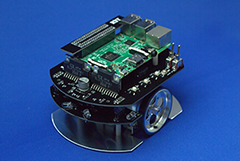
\includegraphics[keepaspectratio, scale=0.8]
      {images/RaspberryPiMouse.png}
 \caption{Example}
 \label{Fig:Example}
\end{figure}

\subsubsection{etc...}
\newpage

%!TEX root = ../thesis.tex

\section{目的}

本研究では,

\subsubsection{etc...}
\newpage

%!TEX root = ../thesis.tex

\section{論文構成}

第1章では,

\subsubsection{etc...}
\newpage

%

%ここにディレクトリのパスを追加していく
\chapter{要素技術}
\label{chap:tectechnology}
%
%\input{introduction/preface}
%
%!TEX root = ../thesis.tex

\section{リーダフォロワ}

第1章では,

\subsubsection{etc...}
\newpage

%

%% Back Matter
\backmatter{}
%
%!TEX root = ../thesis.tex
%\bibliographystyle{plain}
\bibliographystyle{junsrt}
%\bibliography{report}
\nocite{*}
\bibliography{main_bibliography}
%
%!TEX root = ../thesis.tex
\chapter*{付録}
\addcontentsline{toc}{chapter}{付録}

%
%!TEX root = ../thesis.tex
\chapter*{謝辞}
\addcontentsline{toc}{chapter}{謝辞}

本研究を進めるにあたり,1年に渡り, 熱心にご指導を頂いた林原靖男教授に深く感謝いたします.
%


%

\end{document}
